%% LyX 2.3.3 created this file.  For more info, see http://www.lyx.org/.
%% Do not edit unless you really know what you are doing.
\documentclass[english]{article}
\usepackage[latin9]{inputenc}
\usepackage{geometry}
\geometry{verbose,tmargin=2.5cm,bmargin=2.5cm,lmargin=2.5cm,rmargin=2.5cm,headheight=0cm,headsep=0cm}
\usepackage{color}
\usepackage{babel}
\usepackage{graphicx}
\usepackage{float}
\usepackage[unicode=true]
 {hyperref}

\makeatletter

%%%%%%%%%%%%%%%%%%%%%%%%%%%%%% LyX specific LaTeX commands.
%% Because html converters don't know tabularnewline
\providecommand{\tabularnewline}{\\}

\@ifundefined{date}{}{\date{}}
\makeatother

\begin{document}
\title{CSCE 221 - Programming Assignment 4 Report \textbf{(20 points)}}
\maketitle
\begin{center}
{\large{}Due April 14, 2021}{\large\par}
\par\end{center}
\author{First Name:~Clayton~~~~~~~~~~Last Name: ~Kristiansen~~UIN:~328003173}
\author{User Name: kristiansenc~~~~E-mail address:~~kristiansenc@tamu.edu~~~~~~~\medskip{}
}
\begin{quotation}
Please list all sources in the table below including web pages which
you used to solve or implement the current homework. If you fail to
cite sources you can get a lower number of points or even zero, read
more in the Aggie Honor System Office \href{http://aggiehonor.tamu.edu/}{http://aggiehonor.tamu.edu/}\medskip{}
\medskip{}
\end{quotation}
\begin{tabular}{|c|c|c|c|c|c|}
\hline 
\textbf{Type of sources} & ~~~~~~~~~~~~~~~~~~ & ~~~~~~~~~~~~~~~~~~ & ~~~~~~~~~~~~~~~~~~ & ~~~~~~~~~~~~~~~~~~ & ~~~~~~~~~~~~~~~~~~\tabularnewline
\hline 
People & none &  &  &  & \tabularnewline
\hline 
Web pages (provide URL) & none &  &  &  & \tabularnewline
\hline 
Printed material & none &  &  &  & \tabularnewline
\hline 
Other Sources & none &  &  &  & \tabularnewline
\hline 
\end{tabular}
\date{\medskip{}
\medskip{}
}
\begin{quotation}
I certify that I have listed all the sources that I used to develop
the solutions/code to the submitted work.

\textquotedblleft \emph{On my honor as an Aggie, I have neither given
nor received any unauthorized help on this academic work.}\textquotedblright{} 
\end{quotation}
\date{\medskip{}
\medskip{}
}

\begin{tabular}{ccccc}
Your Name (signature) & ~Clayton Kristiansen~ & ~~~~~~~~~~~~~~~~~~~~~ & Date & ~04-14-2021~~\tabularnewline
\end{tabular}\pagebreak{}
\begin{enumerate}
\item The description of the assignment problem.\vfill{}
    
\begin{quotation}
    The assignment was to create 3 different implemenations of a Minimum Priority Queue.
    These implementations would then be tested for functionality, and evaluated in terms
    of efficiency.
\end{quotation}

\item The description of data structures and algorithms used to solve the
problem.
\begin{enumerate}
\item Provide definitions of data structures by using Abstract Data Types
(ADTs) \vfill{}
\begin{enumerate}
    \item The UnsortedMPQ is a vector based class inheriting from the provided MPQ class. It is a
    Minimum Priority Queue that provides functionality for setting items aside and recieving them in
    order of priority.
    \item The SortedMPQ is a linked list based class inheriting from the provided MPQ class. It is a
    Minimum Priority Queue that provides functionality for setting items aside and recieving them in
    order of priority.
    \item The BinaryHeapMPQ is a vector tree based class inheriting from the provided MPQ class. It is a
    Minimum Priority Queue that provides functionality for setting items aside and recieving them in
    order of priority. 
\end{enumerate}
\item Write about the ADTs implementation in C++ (for all the three MPQs).\vfill{}
\begin{enumerate}
    \item The UnsortedMPQ used a vector to store the items in the queue. When insert was called,
    the item was just inserted at the end. When the min or remove min functions were called, the
    methods had to iterate through the vector until the minimum value was found.
    \item The SortedMPQ used a linked list to store the items in the queue. Items were in  sorted
    from highest priority to lowest priority as they were intserted and returned instantly from the
    front of the list when min or remove min was called.
    \item The BinaryHeapMPQ used a vector to store the items in the queue. Items were sorted in the
    binary heap convention as they were inserted to increase efficiency. The vector was arranged such
    that the first element is always the highest priority. 
\end{enumerate}
\item Describe algorithms used to solve the problem. For every MPQ\texttt{
(UnsortedMPQ}, \texttt{SortedMPQ} and \texttt{BinaryHeapMPQ}), list
the MPQ functions (\texttt{remove\_min(), is\_empty(), min(),} and
\texttt{insert()}) and provide their descriptions.\vfill{}
\begin{quotation}
    Every MPQ has the same external functionality of: checking if it is empty, inserting an
    object, returning the highest priority object, and removing the highest priority object.
\end{quotation}
\begin{enumerate}
    \item The UnsortedMPQ
    \begin{enumerate}
        \item is\textunderscore empty() simply checks if the size is equal to zero and returns true if so, false if not.
        \item insert() simply calls the push\textunderscore back method of the vector member to add an object.
        \item min() employs an O(n) search algorithm to find the minimum value, then returns that value.
        \item remove\textunderscore min() does the same as min(), but also removes the min from the vector.
    \end{enumerate}
    \item The SortedMPQ
    \begin{enumerate}
        \item is\textunderscore empty() is the same as above and simply checks if the size is equal to zero and returns true if so, false if not.
        \item insert() uses an iterative algorithm if O(n) to insert each object in the linked list in sorted priority order.
        \item min() returns the first object in the linked list.
        \item remove\textunderscore min() does the same as min(), but also removes the min from the list.
    \end{enumerate}
    \item The BinaryHeapMPQ
    \begin{enumerate}
        \item is\textunderscore empty() is again the same and simply checks if the size is equal to zero and returns true if so, false if not.
        \item insert() will insert the new object at the end of the vector member. Then, a function called up\textunderscore heap() on the new node
        that continually compares the current node to it's parent. If the current node is less than the parent, they are swapped, and the
        check begins again for the new parent.
        \item min() returns the object at the front of the vector. 
        \item remove\textunderscore min() does the same as min(), but also removes the min from the vector. It also moves the node at the end of
        vector to the front and calls a function called down\textunderscore heap() on it that will continually swap that "node" with whatever child
        is the most less than itself until both of its children are greater than itself.
    \end{enumerate}
\end{enumerate}
\item Show the time complexity analysis for the following. Time complexity
analysis means providing a \textbf{basic runtime function/recurrence
relation}, \textbf{solution for recurrence relation with steps (wherever
needed)} and a \textbf{Big-O} Notation:
\begin{enumerate}
\item \textbf{Best, worst, and average case} of each of the MPQ functions
(\texttt{\textbf{remove\_min(), is\_empty(), min(),}}\textbf{ and
}\texttt{\textbf{insert()}}) for \texttt{\textbf{UnsortedMPQ.}} (Note:
Some functions may have same runtimes for all the cases. In that case,
write the answer only once and mention that the runtime applies to
all the cases.).\vfill{}
\begin{enumerate}
    \item \textbf{remove\textunderscore min()}
    \begin{quotation}
        \item Best case (must always iterate through all elements to determine min)
        \begin{equation}
            runtime: n+4
        \end{equation}
        \begin{equation}
            O(n)
        \end{equation}
        \item Worst case (same as best)
        \item Average case (same as best)
    \end{quotation}
    \item \textbf{is\_empty()}
    \begin{quotation}
        \item Best case (simply checks equality of two items
        \begin{equation}
            runtime: 2
        \end{equation}
        \begin{equation}
            O(1)
        \end{equation}
        \item Worst case (same as best)
        \item Average case (same as best)
    \end{quotation}
    \item \textbf{min()}
    \begin{quotation}
        \item Best case (same exact function as remove\_min() simply without the removal (which was O(1)))
        \begin{equation}
            runtime: n+1
        \end{equation}
        \begin{equation}
            O(n)
        \end{equation}
        \item Worst case (same as best)
        \item Average case (same as best)
    \end{quotation}
    \item \textbf{insert()}
    \begin{quotation}
        \item Best case (simply calls push\_back() on the vector which is O(1))
        \begin{equation}
            runtime: 3
        \end{equation}
        \begin{equation}
            O(1)
        \end{equation}
        \item Worst case (same as best)
        \item Average case (same as best)
    \end{quotation}
\end{enumerate}

\begin{enumerate}
\item Provide an \textbf{example for} \textbf{best, worst, and average case}
for \texttt{\textbf{UnsortedMPQ}}. 
\begin{quotation}
    In terms of best/average/worst case insertion or removal for UnsortedMPQ, there
    is no different between input sets. The insert is always O(1) and the min functions
    must always search through every element to gurantee it is the minumum. 
\end{quotation}

\end{enumerate}
\item \textbf{Best, worst, and average case} of each of the MPQ functions
(\texttt{\textbf{remove\_min(), is\_empty(), min(),}}\textbf{ and
}\texttt{\textbf{insert()}}) for \texttt{\textbf{SortedMPQ.}} (Note:
Some functions may have same runtimes for all the cases. In that case,
write the answer only once and mention that the runtime applies to
all the cases).\vfill{}

\begin{enumerate}
    \item \textbf{remove\textunderscore min()}
    \begin{quotation}
        \item Best case (only needs to remove the first element)
        \begin{equation}
            runtime: 3
        \end{equation}
        \begin{equation}
            O(1)
        \end{equation}
        \item Worst case (same as best)
        \item Average case (same as best)
    \end{quotation}
    \item \textbf{is\_empty()}
    \begin{quotation}
        \item Best case (simply checks equality of two items
        \begin{equation}
            runtime: 2
        \end{equation}
        \begin{equation}
            O(1)
        \end{equation}
        \item Worst case (same as best)
        \item Average case (same as best)
    \end{quotation}
    \item \textbf{min()}
    \begin{quotation}
        \item Best case (same exact function as remove\_min() simply without the removal (which was O(1)))
        \begin{equation}
            runtime: 2
        \end{equation}
        \begin{equation}
            O(1)
        \end{equation}
        \item Worst case (same as best)
        \item Average case (same as best)
    \end{quotation}
    \item \textbf{insert()}
    \begin{quotation}
        \item Best case (element to be inserted is smaller than the first element)
        \begin{equation}
            runtime: 3
        \end{equation}
        \begin{equation}
            O(1)
        \end{equation}
        \item Worst case (element to be inserted is greater than all elements currently in the MPQ)
        \begin{equation}
            runtime: n+4
        \end{equation}
        \begin{equation}
            O(n)
        \end{equation}
        \item Average case (element to be inserted is the average off all the elements in the MPQ)
        \begin{equation}
            runtime: n/2+4
        \end{equation}
        \begin{equation}
            O(n)
        \end{equation}
    \end{quotation}
\end{enumerate}

\begin{enumerate}
\item Provide an \textbf{example for} \textbf{best, worst, and average case}
for \texttt{\textbf{SortedMPQ}}.
\end{enumerate}

\begin{quotation}
    Best case (for insert): \{4, 5, 6, 7, 8\} insert 3\\
    Worst case (for insert): \{4, 5, 6, 7, 8\} insert 9\\
    Average case (for insert): \{4, 5, 6, 8, 9, 10\} insert 7 
\end{quotation}

\item \textbf{Best, worst, and average case} of each of the MPQ functions
(\texttt{\textbf{remove\_min(), is\_empty(), min(),}}\textbf{ and
}\texttt{\textbf{insert()}}) for \texttt{\textbf{BinaryHeapMPQ.}}
(Note: Some functions may have same runtimes for all the cases. In
that case, write the answer only once and mention that the runtime
applies to all the cases).

\begin{enumerate}
    \item \textbf{remove\textunderscore min()}
    \begin{quotation}
        \item Best case (the heap has only one element)
        \begin{equation}
            runtime: 2
        \end{equation}
        \begin{equation}
            O(1)
        \end{equation}
        \item Worst case (rightmost element is largest element)
        \begin{quotation}
            The number of comparisons required to delete a node in 
            the a heap is proportional to the length 
            of the path the swapped item travels as it moves down. 
            Since the binary tree is dense, this path length is O(log(n)) 
            with n nodes. Therefore, the runtime efficiency delete is O(log(n)).
            I also implemented this function iteratively.
        \end{quotation}
        \begin{equation}
            runtime: 3*log(n)+4
        \end{equation}
        \begin{equation}
            O(log(n))
        \end{equation}
        \item Average case (rightmost element is average of all elements)
        \begin{equation}
            runtime: 3*log(n/2)+4
        \end{equation}
        \begin{equation}
            O(log(n))
        \end{equation}
    \end{quotation}
    \item \textbf{is\_empty()}
    \begin{quotation}
        \item Best case (simply checks equality of two items
        \begin{equation}
            runtime: 2
        \end{equation}
        \begin{equation}
            O(1)
        \end{equation}
        \item Worst case (same as best)
        \item Average case (same as best)
    \end{quotation}
    \item \textbf{min()}
    \begin{quotation}
        \item Best case (same exact function as remove\_min() simply without the removal (which was O(1)))
        \begin{equation}
            runtime: 2
        \end{equation}
        \begin{equation}
            O(1)
        \end{equation}
        \item Worst case (same as remove\_min())
        \begin{equation}
            runtime: 3*log(n)+4
        \end{equation}
        \begin{equation}
            O(log(n))
        \end{equation}
        \item Average case (same as remove\_min())
        \begin{equation}
            runtime: 3*log(n/2)+4
        \end{equation}
        \begin{equation}
            O(log(n))
        \end{equation}
    \end{quotation}
    \item \textbf{insert()}
    \begin{quotation}
        \item Best case (element to be inserted is greater than all other elements)
        \begin{equation}
            runtime: 3
        \end{equation}
        \begin{equation}
            O(1)
        \end{equation}
        \begin{quotation}
            The number of comparisons required to insert a node in 
            the a heap is proportional to the length 
            of the path the inserted item travels as it moves up. 
            Since the binary tree is dense, this path length is O(log(n)) 
            with n nodes. Therefore, the runtime efficiency delete is O(log(n)).
            I also implemented this function iteratively.
        \end{quotation}
        \item Worst case (element to be inserted is less than than all elements currently in the MPQ)
        \begin{equation}
            runtime: 4*log(n)+5
        \end{equation}
        \begin{equation}
            O(log(n))
        \end{equation}
        \item Average case (element to be inserted is the average off all the elements in the MPQ)
        \begin{equation}
            runtime: 4*log(n/2)+5
        \end{equation}
        \begin{equation}
            O(log(n))
        \end{equation}
    \end{quotation}
\end{enumerate}

\begin{enumerate}
\item Provide an \textbf{example for} \textbf{best, worst, and average case}
for \texttt{\textbf{BinaryHeapMPQ}}. 
\begin{quotation}
    Best case (for insert): \{4, 5, 6, 7, 8\} insert 9\\
    Worst case (for insert): \{4, 5, 6, 7, 8\} insert 3\\
    Average case (for insert): \{4, 5, 6, 8, 9, 10\} insert 7\\ 
    Best case (for min): \{4\}\\
    Worst case (for min): \{4, 5, 6, 7, 8\}\\
    Average case (for min): \{4, 5, 6, 8, 9, 7\}
\end{quotation}

\pagebreak{}
\end{enumerate}
\end{enumerate}
\end{enumerate}
\item A C++ organization and implementation of the problem solution 
\begin{enumerate}
\item Provide a list and description of classes or interfaces used by a
program such as classes used to implement the data structures or exceptions.
\begin{enumerate}
    \item MPQ - Minimum priority queue, ADT that allows for storage, and access, of items with accordance to their priority.
    \item BinaryHeap - A heap structure based off a vector that treats the vector like a binary tree where each parent must be > their child. 
    \item UnsortedMPQ - MPQ implemented with vector.
    \item SortedMPQ - MPQ implemented with linked list.
    \item BinaryHeapMPQ - MPQ implemented with binary heap.
    \item RuntimeException - Exception thrown when an error is encountered during runtime.
\end{enumerate}
\item Provide features of the C++ programming paradigms like Inheritance
or Polymorphism in case of object oriented programming, or Templates
in the case of generic programming used in your implementation. 
\begin{enumerate}
    \item Inheritance - All the MPQ classes in this project are inherited from the MPQ class
    \item Templates - Every class and helper function is templatized to allow each
    MPQ to handle different types of (already comparable) data.
\end{enumerate}
\end{enumerate}
\item A user guide description how to navigate your program with the instructions
how to: 
\begin{enumerate}
\item compile the program: specify the directory and file names, etc.
\begin{quotation}
    Open a Linux terminal to the directory containing the makefile. Type "make all" to compile the program.
    This creates the "test" file
\end{quotation}
\item run the program: specify the name of an executable file.
\begin{quotation}
    Type "make run" to run the program. This runs the file "test". You may also type "./test"
\end{quotation}
\pagebreak{}
\end{enumerate}
\item Specifications and description of input and output formats and files 
\begin{enumerate}
\item The type of files: keyboard, text files, etc (if applicable).
\begin{quotation}
    All input and output files are .txt files. User input is done through the keyboard.
\end{quotation}
\item A file input format: when a program requires a sequence of input items,
specify the number of items per line or a line termination. Provide
a sample of a required input format.
\begin{quotation}
    The .txt files must be formatted with 3 integers (one CPU task) per line.
    The integers are ID, Length, and Priority. They are to be seperated by spaces with a newline at the end.
    \begin{quotation}
        Ex:\\
        6	2	15\\
        3	8	3\\
        2	10	-16\\
        8	3	-3\\
        4	7	-16\\
        9	9	-3
    \end{quotation}  
\end{quotation}
\item Discuss possible cases when your program could crash because of incorrect
input (a wrong file name, strings instead of a number, or such cases
when the program expects 10 items to read and it finds only 9.)
\begin{quotation}
    The program is quite robust, if it encounters an unexpected length it will always read as far as possible
    before completing its task (it won't crash). It wil throw an exception, however, if operations are attempted
    to be performed on an empty MPQ, or if an input file does not exist.
\end{quotation}
\end{enumerate}
\item Provide types of exceptions and their purpose in your program (Answer
only to the ones that are applicable for this assignment).
\begin{enumerate}
\item logical exceptions (such as deletion of an item from an empty container,
etc.).
\begin{quotation}
    Logical exceptions are thrown when a requested input file does not exist,
    or when an empty MPQ is operated on with either min() or remove\_min().
\end{quotation}
\item runtime exception (such as division by $0$, etc.)
\begin{quotation}
    These exeptions are not currently explicitly handled by the program.
\end{quotation}
\end{enumerate}
\item Include evidence of your testing by providing screenshots. Screenshots
should show execution of the 5 main methods \texttt{(unsortedmpq-main.cpp,
sortedmpq-main.cpp, main.cpp, cpu-job-main.cpp, binaryheap-mpq-main.cpp).}
\begin{figure}[H]
    \centering
    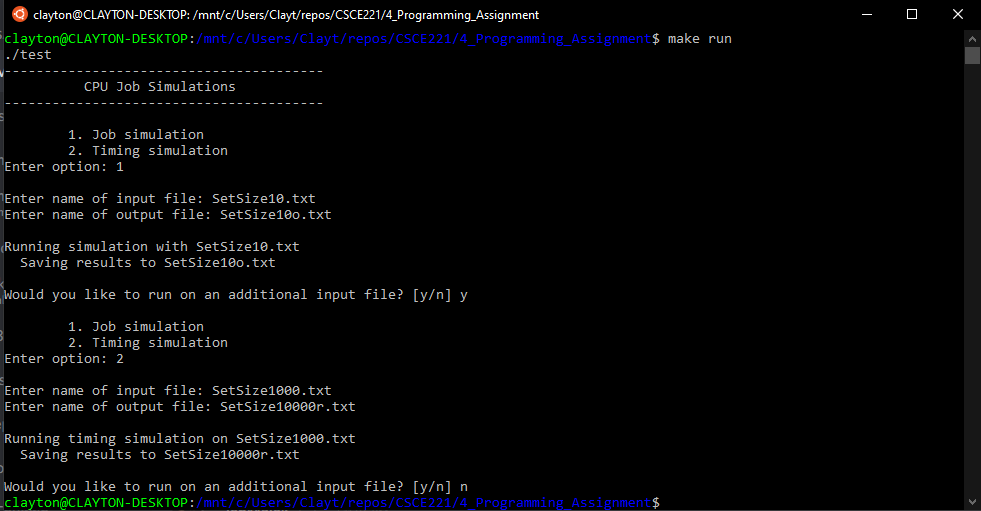
\includegraphics[width=0.8\linewidth]{Main.png}
    \caption{CPU Tests}%
    \label{fig:1}
 \end{figure}
 \begin{figure}[H]
    \centering
    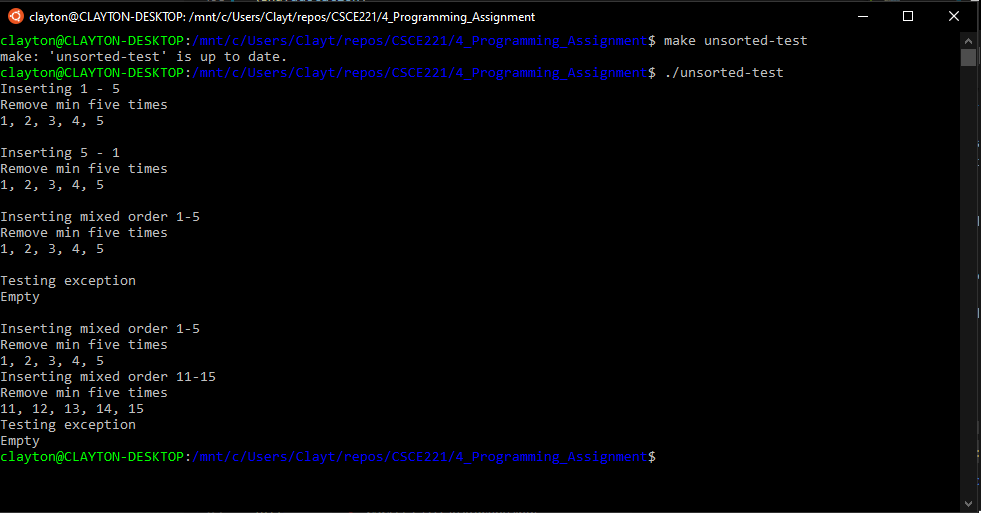
\includegraphics[width=0.8\linewidth]{Unsorted-test.png}
    \caption{Unsorted Tests}%
    \label{fig:2}
 \end{figure}
 \begin{figure}[H]
    \centering
    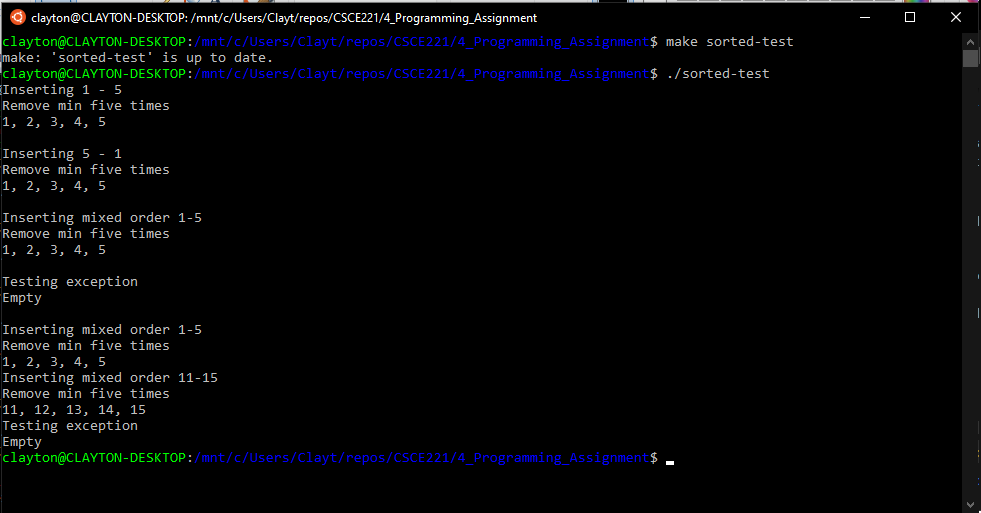
\includegraphics[width=0.8\linewidth]{Sorted-test.png}
    \caption{Sorted Tests}%
    \label{fig:3}
 \end{figure}
 \begin{figure}[H]
    \centering
    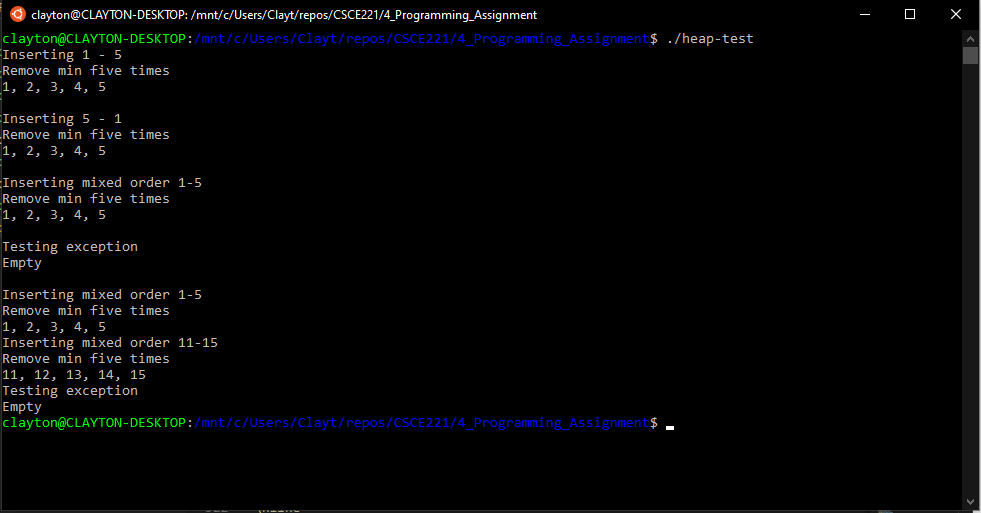
\includegraphics[width=0.8\linewidth]{Heap-test.png}
    \caption{BinaryHeap tests}%
    \label{fig:4}
 \end{figure}


\item Provide graphs and data tables of your CPU timing simulation results.
Graph should be plotted for \textbf{runtime vs. input size}. The input
sizes are 4, 10, 100, and 1,000. To obtain this data, compile and
run \texttt{main.cpp}. Choose option ``2. Timing Simulation''. Provide
the input file name (SetSize4.txt) and output filename. After execution,
you will find the output file in ``OutputFiles'' folder. The timing
for all the three MPQ implementations will be displayed. Fill it in
the following table and plot it as a \textbf{graph}.

\begin{tabular}{|c|c|c|c|}
\hline 
 & \multicolumn{3}{c|}{Runtime}\tabularnewline
\hline 
Input Sizes & Unsorted MPQ & Sorted MPQ & Binary heap MPQ\tabularnewline
\hline 
4 (SetSize4.txt) & 0.0094 & 0.0092 & 0.0082\tabularnewline
\hline 
10 (SetSize10.txt) & 0.0467 & 0.0102 & 0.0257\tabularnewline
\hline 
100 (SetSize100.txt) & 0.3477 & 0.1953 & 0.1092\tabularnewline
\hline 
1000 (SetSize1000.txt) & 17.1037 & 10.6245 & 1.0095\tabularnewline
\hline 
\end{tabular}

\begin{figure}[H]
    \centering
    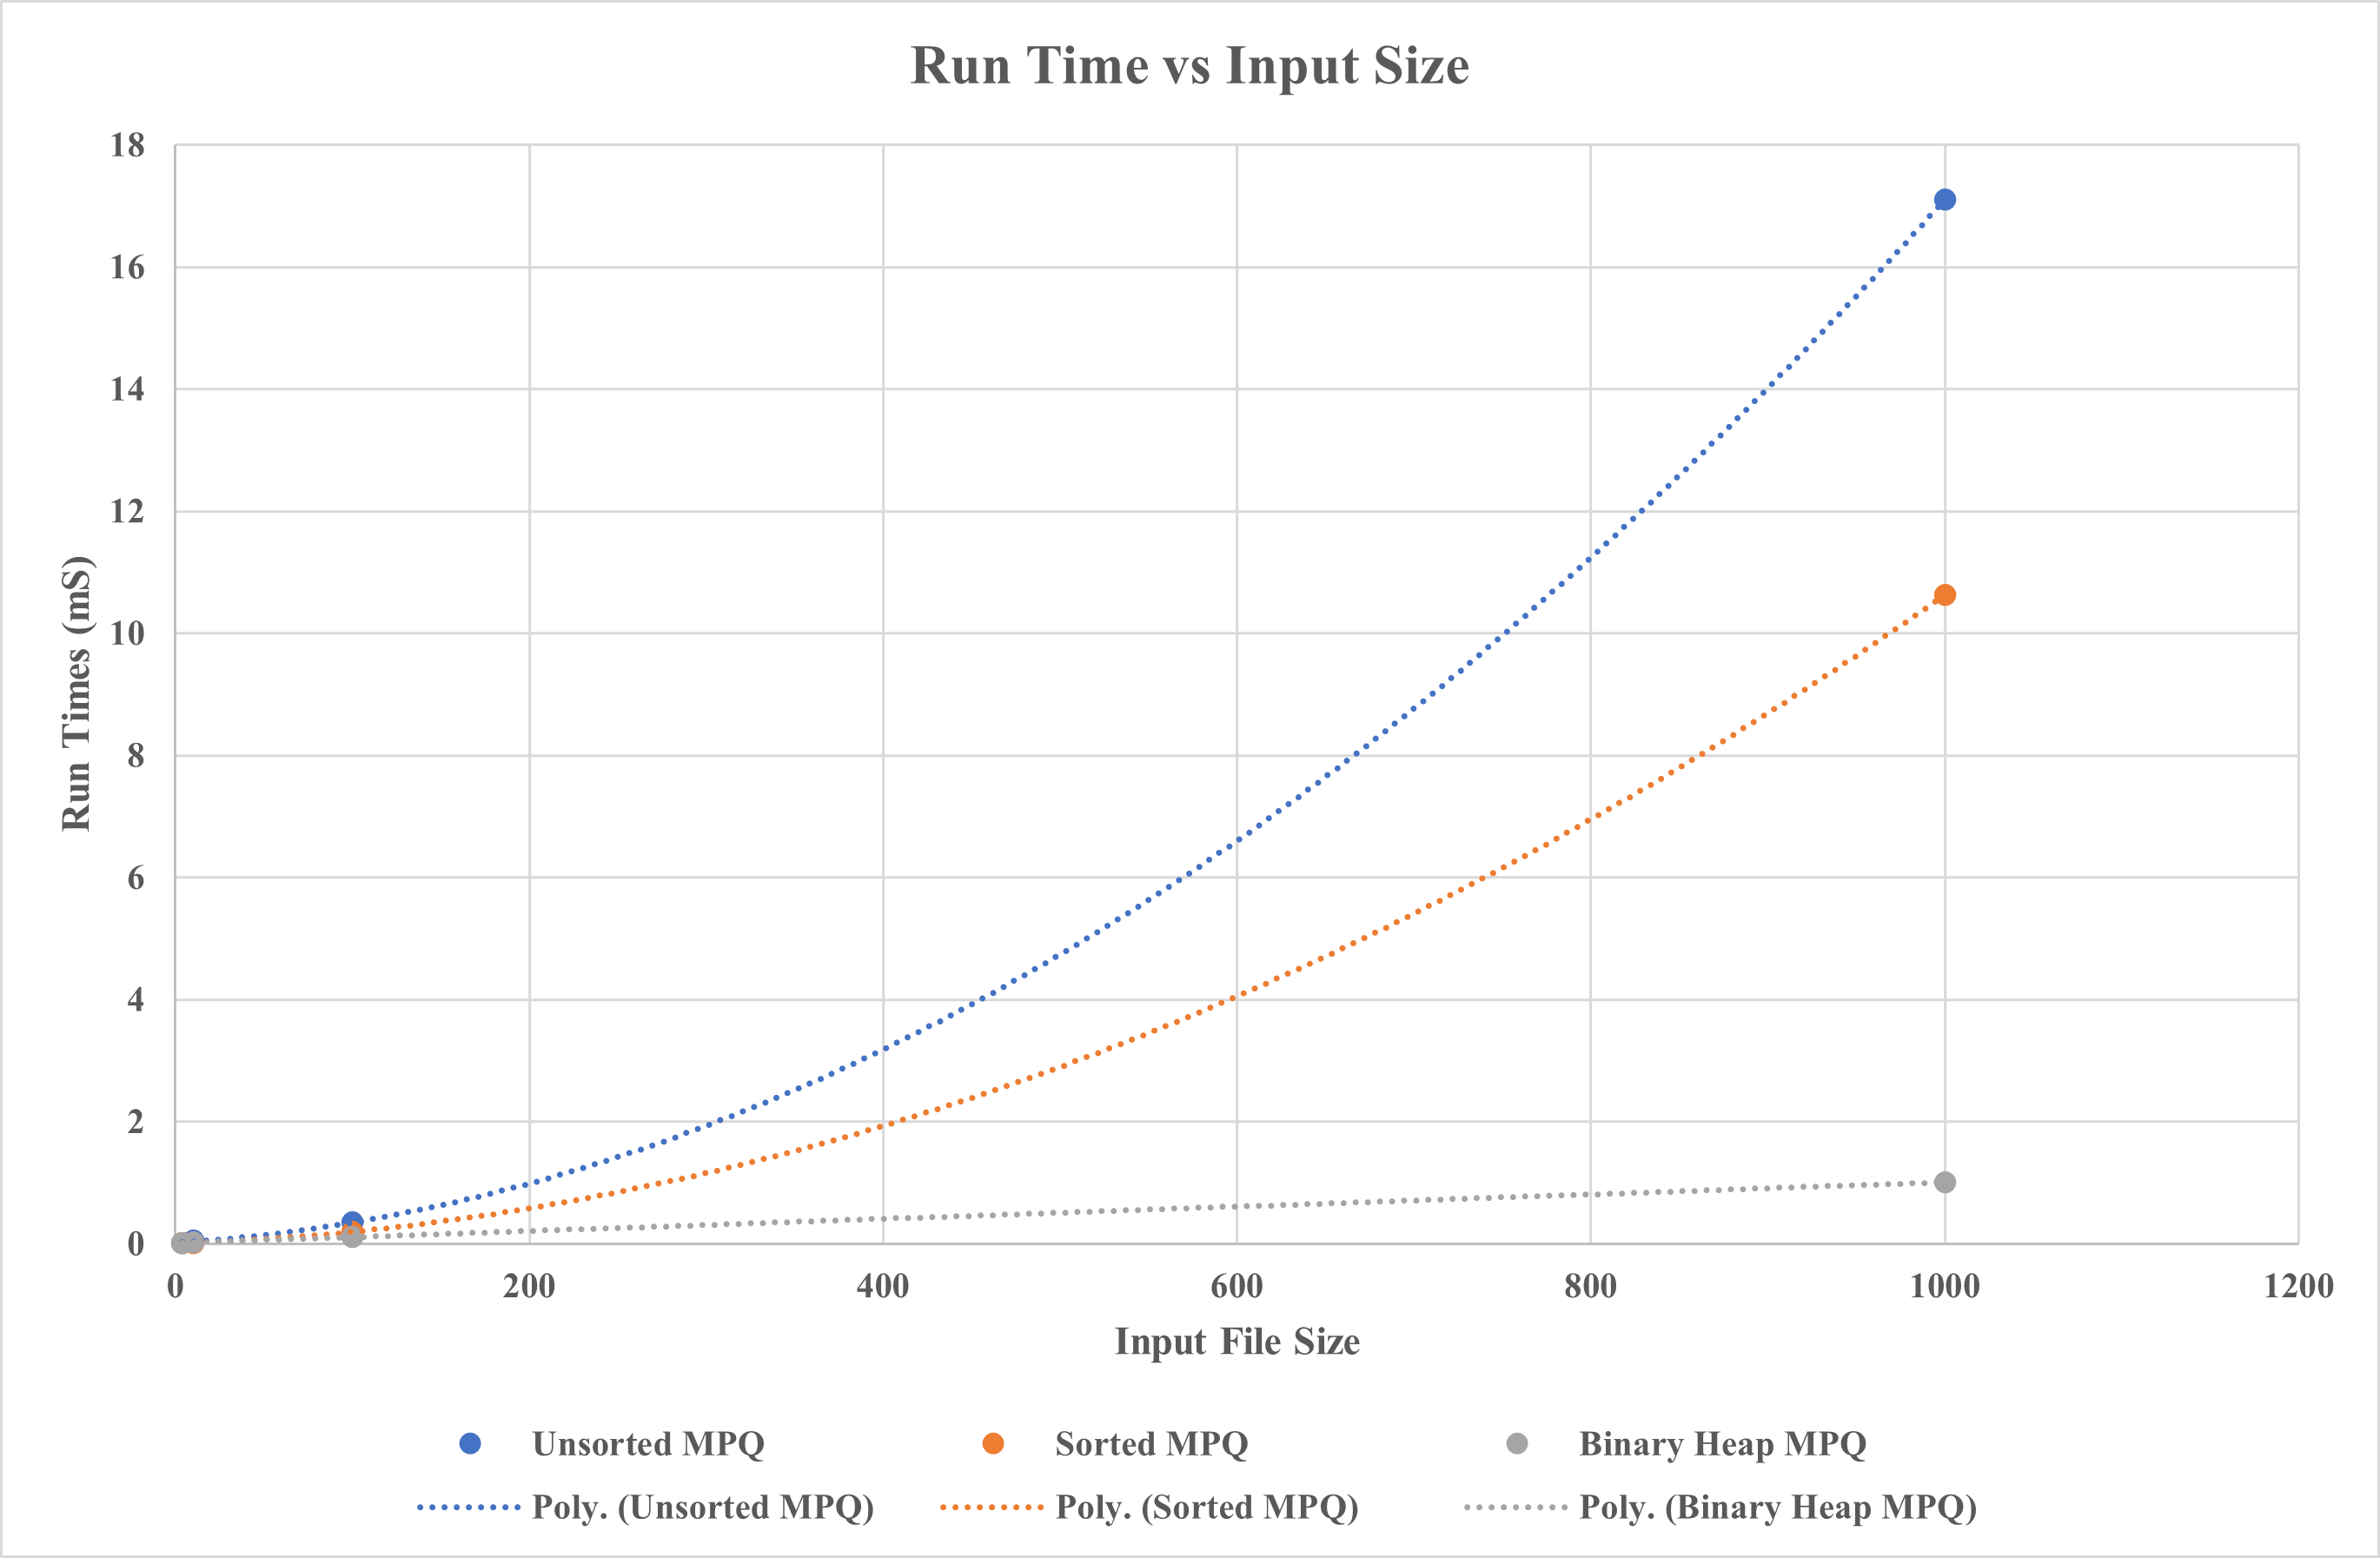
\includegraphics[width=0.8\linewidth]{Graph.png}
    \caption{CPU timing simulation results graph}%
    \label{fig:5}
 \end{figure}

\end{enumerate}

\end{document}
